% arara: pdflatex
% arara: biber
% arara: pdflatex
% arara: pdflatex

\documentclass[12pt, notitlepage, twoside]{report}



% Document Metafiles (Do Not Reorder!) ===================================== %
% Dissertation Template Preamble %
% ============================== %

% Declare packages here

\usepackage{subfiles}
\usepackage{geometry}
\usepackage{amsmath}
\usepackage{pgfkeys}
\usepackage{sectsty}
\usepackage{graphicx}
\usepackage{lipsum}
\usepackage[english]{babel}
\usepackage[utf8]{inputenc}
\usepackage[backend=biber,style=numeric,sorting=nyt]{biblatex}
\usepackage[toc]{appendix}
\usepackage{setspace}
\usepackage{titlesec}
\usepackage{csquotes}
\usepackage{hyperref}
\usepackage{booktabs}
\usepackage{physics}
\usepackage{amsmath}
\usepackage{tikz}
\usepackage{mathdots}
\usepackage{yhmath}
\usepackage{cancel}
\usepackage{color}
\usepackage{siunitx}
\usepackage{array}
\usepackage{multirow}
\usepackage{amssymb}
\usepackage{gensymb}
\usepackage{tabularx}
\usepackage{extarrows}
\usepackage{booktabs}
\usetikzlibrary{fadings}
\usetikzlibrary{patterns}
\usetikzlibrary{shadows.blur}
\usetikzlibrary{shapes}



% Moves table captions to the top to comply with formatting check: https://tex.stackexchange.com/questions/22751/how-to-force-table-caption-on-top
\usepackage{float}
\floatstyle{plaintop}
\restylefloat{table}


\newif\ifsidenote
\newif\iffigures
\newif\iftables

% Template Structure File %
% ======================= %

% Use this geometry for the frontmatter
\geometry{width=8.5in,
          height=11in,
          left=1in,
          right=1in,
          top=1in,
          bottom=1.25in}

% Overall typography and aesthetics --------------------

% Not double-spaced.
  \setstretch{1.1}
  \textfloatsep 0.75in

% Better font
\usepackage[T1]{fontenc}
\usepackage[osf]{ebgaramond}

% Makes widows and orphans illegal.
\usepackage[all]{nowidow}
% This prevents unwanted spaces between paragraphs
\raggedbottom

% Word spacing and letter spacing
\usepackage[activate={true,nocompatibility},final,tracking=true,kerning=true,spacing=true,factor=1100,stretch=10,shrink=10]{microtype}
% activate={true,nocompatibility} - activate protrusion and expansion
% final - enable microtype; use "draft" to disable
% tracking=true, kerning=true, spacing=true - activate these techniques
% factor=1100 - add 10% to the protrusion amount (default is 1000)
% stretch=10, shrink=10 - reduce stretchability/shrinkability (default is 20/20)
% See http://www.khirevich.com/latex/microtype/
\microtypecontext{spacing=nonfrench} % suppresses some warnings

% End typography ----------------------------------------

\addbibresource{metafiles/dissertation.bib}

\chapterfont{\centering\normalfont\nohang\textsc} %Centering Chapter Headers





% Document Structure Options =============================================== %
\sidenotetrue
%\sidenotefalse
\figurestrue
% \figuresfalse
\tablestrue
% \tablesfalse

% If you want sidenotes, we'll load some additional packages. Nothing for you to worry about.

\ifsidenote
  \usepackage{marginfix}
  \usepackage{sidenotes}
  \usepackage{ragged2e} % A better version of \raggedright and will prevent overly short lines in sidenotes: https://texfaq.org/FAQ-ragright
  \renewcommand{\footnote}[1]{\sidenote{\RaggedRight\footnotesize #1}}
  \renewcommand{\footnotetext}[1]{\sidenotetext{\raggedright\footnotesize #1}}
\fi

\ifsidenote
  % We'll now switch to the sidenote layout.
  \newgeometry{
    height = 11in,
    width = 8.5in,
    includemp = true,
    top = 1in,
    bottom = 1.25in,
    bindingoffset = 0.25in,
    inner = 1in,
    marginparsep = 0.125in,
    marginparwidth = 1.5in,
    outer = 0.75in
  }

  \renewcommand{\footnote}[1]{\sidenote{\RaggedRight\footnotesize #1}}
  \renewcommand{\footnotetext}[1]{\sidenotetext{\raggedright\footnotesize #1}}
% If you want FOOTNOTES instead of sidenotes.
\else
  % Do nothing. We're all good.
\fi



%% COVER PAGE


\begin{document}

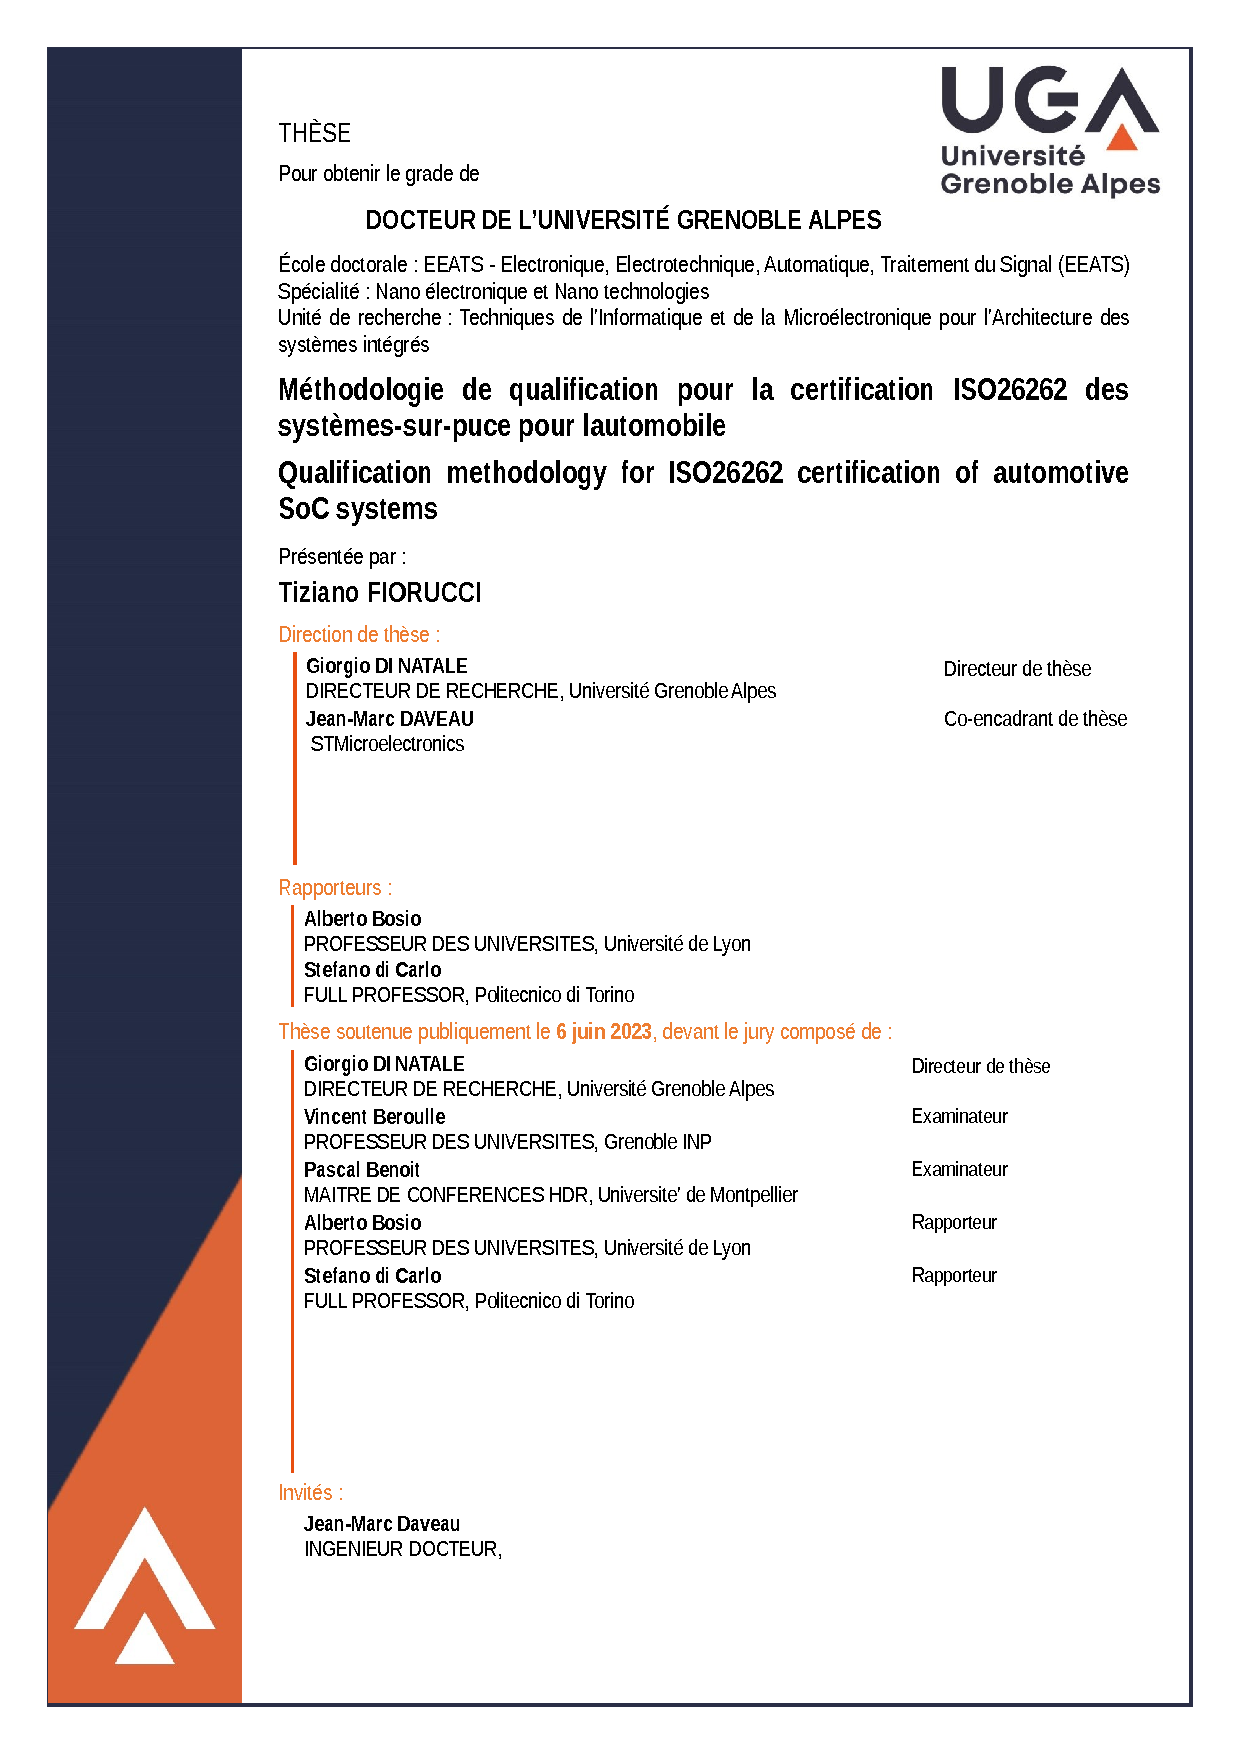
\includepdf[pages=-]{couverture_these.pdf}
% Title and Author Settings ================================================ %



\newcommand{\doctitle}{Qualification methodology for ISO26262
certification of automotive SoC systems}
\newcommand{\docauthor}{Tiziano Fiorucci}


%--------------------------ABSTRACT---------------------------%
\newcommand{\makeabstract}[1]{%
\begingroup
\newpage

\thispagestyle{empty}
\vspace*{18pt}
\begin{center}
  \textsc{\Large{\doctitle}}\\[18pt]
  by\\[18pt]
  \textsc{\Large\docauthor}\\[12pt]
  (Under the Direction of Giorgio di Natale)\\[12pt]
  \textsc{Abstract}
\end{center}

#1

\thispagestyle{empty}

\begin{list}{\textsc{Index words:\hfill}}{\labelwidth 1.2in\leftmargin 1.4in\labelsep 0.2in}
  \item \begin{flushleft}
    [FMEA, ISO26262, System on Chip, Reliability, Functional Safety]
  \end{flushleft}
\end{list}
\endgroup}

\makeabstract{This thesis proposes to set up a flow and a methodology of ISO26262 certification for system-type integrated circuits on a digital chip dedicated to driving. These circuits are generally composed of several Intellectual Properties, IPs, dedicated to different functions such as communication or processing of information from sensors (camera, lidar ...), real-time system, vision and imaging, system management (operating system), security.
The ISO26262 methodology requires the extraction of a number of metrics related to the resilience of the system to single and multiple faults as well as the effectiveness of countermeasures (detection, reporting and correction of errors) and failure modes. The extraction of failure metrics from fault trees is a method known and documented in the literature. Nevertheless, its application has often been limited to macroscopic electromechanical systems such as a car, actuator or sensor chains. On the other hand, these methods are rarely applied in the field of automotive SoCs where the extraction of metrics is still largely manual (usually using a spreadsheet) and dependent on an expert, and where the verification of the effectiveness of countermeasures is best done by targeted fault injection on a few sub-parts of the complete system or irradiation under a particle beam.
This thesis proposes to develop a reliability metrics extraction methodology based on fault injection per block as well as composition methods to obtain the metrics at the level of the complete system. The first part of the thesis will be devoted to the study of the bibliography on the construction of fault trees, the ISO26262 standard and the declination of the different reliability metrics in the case of a digital SoCs type system. The extraction of metrics at the block level will be based on 2 different methods, one analytical based on probabilities, the other experimental based on fault injection. The aim is not to develop new probability codes or fault injection tools but to develop a methodology to use them in the context of a SoC to obtain the desired data. The second part of the thesis will concern the composition of the data obtained at the functional block level in order to obtain the ISO26262 metrics at the system level (SoC). It will be a matter of developing a composition method adapted in particular to the characteristics of SoCs (communicating system, performing calculations that must react in real time, ...) and to the fault models that characterize them or imposed by the ISO26262 standard. The third part of the thesis concerns the application of the developments described in the previous paragraph to an SoC-type system and the verification of the results obtained.



\paragraph{French Translation} 
Cette thèse propose de mettre en place un flux et une méthodologie de certification ISO26262 pour les circuits intégrés de type système sur une puce numérique dédiée à la conduite. Ces circuits sont généralement composés de plusieurs propriétés intellectuelles, IP, dédiées à différentes fonctions telles que la communication ou le traitement d'informations provenant de capteurs (caméra, lidar...), le système en temps réel, la vision et l'imagerie, la gestion du système (système d'exploitation), la sécurité. La méthodologie ISO26262 nécessite l'extraction d'un certain nombre de métriques liées à la résilience du système face aux pannes simples et multiples, ainsi qu'à l'efficacité des contre-mesures (détection, signalement et correction des erreurs) et modes de défaillance. L'extraction des métriques d'échec à partir des arbres de défaillance est une méthode connue et documentée dans la littérature. Néanmoins, son application a souvent été limitée aux systèmes électromécaniques macroscopiques tels qu'une voiture, un actionneur ou des chaînes de capteurs. D'autre part, ces méthodes sont rarement appliquées dans le domaine des SoC automobiles où l'extraction des métriques est encore largement manuelle (généralement à l'aide d'un tableur) et dépendante d'un expert, et où la vérification de l'efficacité des contre-mesures est mieux effectuée par injection de fautes ciblée sur quelques sous-parties du système complet ou par irradiation sous un faisceau de particules. Cette thèse propose de développer une méthodologie d'extraction de métriques de fiabilité basée sur l'injection de fautes par bloc ainsi que des méthodes de composition pour obtenir les métriques au niveau du système complet. La première partie de la thèse sera consacrée à l'étude de la bibliographie sur la construction d'arbres de défaillance, la norme ISO26262 et la déclinaison des différentes métriques de fiabilité dans le cas d'un système SoCs numérique. L'extraction des métriques au niveau du bloc sera basée sur deux méthodes différentes, l'une analytique basée sur les probabilités, l'autre expérimentale basée sur l'injection de fautes. L'objectif n'est pas de développer de nouveaux codes de probabilité ou des outils d'injection de fautes, mais de développer une méthodologie pour les utiliser dans le contexte d'un SoC afin d'obtenir les données souhaitées. La deuxième partie de la thèse concernera la composition des données obtenues au niveau du bloc fonctionnel afin d'obtenir les métriques ISO26262 au niveau du système (SoC). Il s'agira de développer une méthode de composition adaptée en particulier aux caractéristiques des SoCs (système de communication, effectuant des calculs devant réagir en temps réel, ...) et aux modèles de défaillance qui les caractérisent ou imposés par la norme ISO26262.
}%


%--------------------------TITLE PAGE---------------------------%
\newcommand{\maketitlepage}{%
\newpage
\pagenumbering{roman}
\thispagestyle{empty}
\vspace*{18pt}
\begin{center}
  \textsc{\doctitle}\\[18pt]
  by\\[12pt]
  \textsc{\docauthor}\\[8pt]
  \degreesearned

  \vfill
  A \degreetype\ Submitted to the Graduate Faculty of the\\
	University of Grenoble Alpes.\\ [18pt]

  \textsc{\degreetitle\ of \degreename}\\[24pt]
  \textsc{Grenoble, France}\\[18pt]
  \degreeyear
\end{center}}

\newcommand{\degreesearned}{%
B.S., University of Rome "Tor Vergata", 2018\\
B.Sc., University of Rome "Tor Vergata", 2016
}%

\newcommand{\degreetype}{Dissertation}
\newcommand{\degreetitle}{Doctor of Philosophy}
\newcommand{\degreename}{Nano Electronics and Nano Technologies}
\newcommand{\degreeyear}{2023}
\maketitlepage


%--------------------------COPYRIGHT---------------------------%
\newcommand{\makecopyright}[1]{%
\newpage
\thispagestyle{empty}
\vspace*{6.6in}
\begin{center}
  \copyright #1\\
  \docauthor\\
  All Rights Reserved
\end{center}}

\makecopyright{2023}


%--------------------------APPROVAL---------------------------%
\newpage
\thispagestyle{empty}
\vspace*{18pt}
\begin{center}
  \textsc{\doctitle}\\[18pt]
  by\\[18pt]
  \textsc{\docauthor}
\end{center}
\vfill

\begin{flushright}
  \begin{tabular}{ll}
    Major Professor: & Giorgio di Natale \\ [8pt]
    Industrial Advisor: & Jean Marc Daveau \\ [8pt]
    Committee: & Alberto Bosio \\
    & Stefano di Carlo \\
    & Pascal Benoit \\
    & Vincent Berouille \\
  \end{tabular}
\end{flushright}

\vspace*{3cm}

\begin{flushleft}
  Electronic Version Approved\\[12pt]
\end{flushleft}
\vspace*{1.5cm}

%QUOTE =====================================

\subfile{subfiles/quote}


% Dedication ============================================================== %
\subfile{subfiles/dedication}

% Acknowledgements ======================================================== %
\subfile{subfiles/acknowledgements}

% Table of Contents ======================================================= %
\setcounter{tocdepth}{1}
\tableofcontents

\iffigures
\addcontentsline{toc}{chapter}{\listfigurename}
\listoffigures
\fi

\iftables
\addcontentsline{toc}{chapter}{\listtablename}
\listoftables
\fi

\clearpage
\pagenumbering{arabic}

% Document Body =========================================================== %
% ------------------------------------------------------------------------- %
\subfile{subfiles/soa}
\subfile{subfiles/chapter1}
\subfile{subfiles/problem_and_contribution.tex}
\subfile{subfiles/chapter2}
\subfile{subfiles/chapter3}
\subfile{subfiles/Analysis/intro.tex}
\subfile{subfiles/chapter5}
\subfile{subfiles/conclusion}
% ------------------------------------------------------------------------- %
% ========================================================================= %


%-----------------------APPENDICES----------------------------%
\begin{appendices}
  \subfile{subfiles/appendices}
\end{appendices}

%-----------------------BIBLIOGRAPHY---------------------------%
\newpage
\addcontentsline{toc}{chapter}{Bibliography} %add bib to the TOC
\printbibliography[title={Bibliography}]

\end{document}
